\documentclass[border=1mm]{standalone}
% \usepackage[margin=2.5cm]{geometry}

\usepackage{graphicx,tikz,tikz-layers} 
\usetikzlibrary{decorations.markings,calc,positioning,arrows,shapes.geometric,arrows.meta}

\colorlet{myred}{red!80!black}
\colorlet{myblue}{blue!80!black}
\colorlet{mybluee}{myblue!80!black}
\colorlet{mygreen}{green!60!black}
\colorlet{myorange}{orange!70!red!60!black}
\colorlet{mydarkred}{red!20!black}
\colorlet{mydarkblue}{blue!40!black}
\colorlet{mydarkgreen}{green!20!black}


\begin{document}

% \resizebox{\textwidth}{!}{
\tikz[font=\small,scale=1, every node/.style={outer sep=0pt, inner sep=0pt, align=center}, w/.style={minimum width=#1},h/.style={minimum height=#1},s/.style={minimum size=#1}, eu/.style={shorten >=#1},ed/.style={shorten <=#1},line join=round]
{
\tikzset{>={Latex[length=1.5mm, width=1.25mm]}}

\node[draw, thick, label={[label distance=2mm, font=\scriptsize]below:1. Input image}] (im) {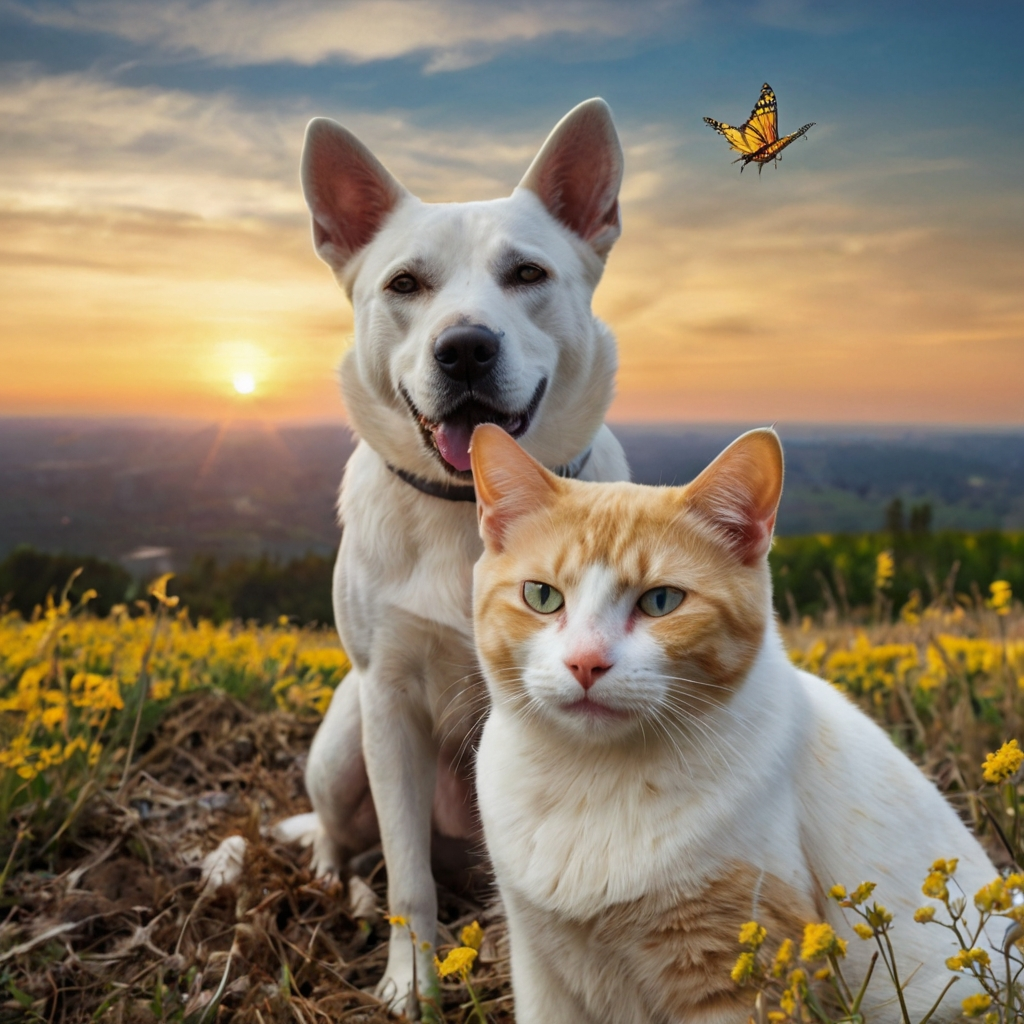
\includegraphics[width=2.2cm]{images/cat&dog.jpg}};

\node[draw, thick, right=.75cm of im, label={[label distance=2mm, font=\scriptsize]below:2. Extraction region\\proposals ($\sim\! 2k$)}] (im1) {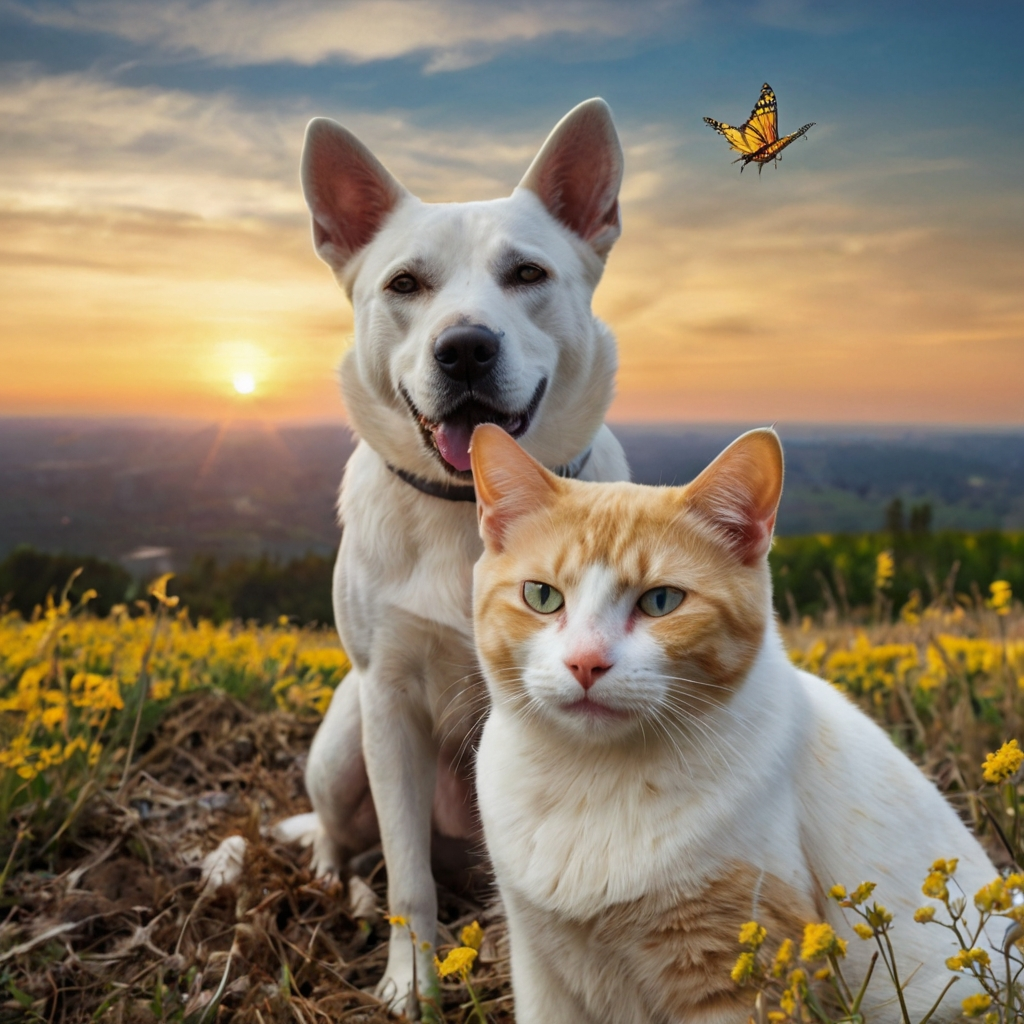
\includegraphics[width=2.2cm]{images/cat&dog.jpg}};

\node[draw, red, ultra thick, right=.75cm of im1] (im2) {
\includegraphics[width=1cm]{images/cat&dog_cropped.jpg}};

\node[draw, right=.75cm of im2, s=1cm, fill=white, yshift=1mm] (a0) {};
\node[draw, s=1cm, fill=white] (a1) at ($(a0)+(.1,-.1)$) {};
\node[draw, s=1cm, fill=white] (a2) at ($(a1)+(.1,-.1)$) {};

\node[draw, s=.5cm, fill=white] (a3) at ($(a2)+(.1,.1)$) {};
\node[draw, thick, s=.5cm] (a33) at ($(im2)+(.1,.1)$) {};

\node[draw, right=.75cm of a0, s=.5cm, fill=white, yshift=1mm] (b0) {};
\node[draw, s=.5cm, fill=white] (b1) at ($(b0)+(.2,-.2)$) {};
\node[draw, s=.5cm, fill=white] (b2) at ($(b1)+(.2,-.2)$) {};

\node[w=.7cm, h=1cm, right=.5cm of b1] (c1) {};
\draw (c1.north west)--($(c1.north west)+(0,-.3)$)--(c1.south east)--($(c1.south east)+(0,.3)$)--cycle;
\node[w=.7cm, h=1cm, right=-.1cm of c1] (c2) {};
\draw (c2.north west)--($(c2.north west)+(0,-.3)$)--(c2.south east)--($(c2.south east)+(0,.3)$)--cycle;

\node[draw, right=.75cm of c2, w=2.5cm, h=.5cm] (per) {dog? yes.};
\node[draw, above=.5cm of per, w=2.5cm, h=.5cm] (aer) {aeroplane? no.};
\node[draw, below=.5cm of per, w=2.5cm, h=.5cm, label={[label distance=2mm, font=\scriptsize]below:4. Classify regions}] (tvm) {person? no.};

\node[draw, densely dotted, w=4.45cm, h=1.4cm, anchor=north west, label={[label distance=7.5mm, font=\scriptsize]below:3. Compute CNN features}] at ($(a0.north west)+(-.1,.1)$) {};

\node[draw, red, ultra thick, s=1.1cm, xshift=-1mm, yshift=4.5mm] (r1) at (im1.center) {};
\node[draw, red, ultra thick, s=.45cm, anchor=south east,  xshift=-3.5mm, yshift=17mm] (r2) at (im1.south east) {};
\node[draw, red, ultra thick, w=1.5cm, h=1.1cm, xshift=3.5mm, yshift=-3mm] (r3) at (im1.center) {};
\node[draw, red, ultra thick, s=.45cm, anchor=south east] (r4) at (im1.south east) {};

% Arrows
\draw[->, dashed] (r1) to[out=0, in=180] ($(im2.west)+(0,.3)$);
\draw[->, dashed, gray] (r2) to[out=0, in=180] ($(im2.west)+(0,.1)$);
\draw[->, dashed, gray] (r3) to[out=0, in=180] ($(im2.west)+(0,-.1)$);
\draw[->, dashed, gray] (r4) to[out=0, in=180] ($(im2.west)+(0,-.3)$);

\draw (a33.north east)--(a3.center);
\draw (a33.south east)--(a3.center);

\draw (a3.north east)--(b2.center);
\draw (a3.south east)--(b2.center);

\draw[ed=1mm] ($(a1.east)+(0,.35)$)--($(b1.center)+(-.05,0)$);
\draw[ed=1mm] ($(a1.east)+(0,-.1)$)--($(b1.center)+(-.05,0)$);  

\draw[ed=1mm] ($(a0.east)+(0,.4)$)--($(b0.center)+(-.05,0)$);
\draw[ed=2mm] ($(a0.east)+(0,0)$)--($(b0.center)+(-.05,0)$);  

\draw (b1.35)--(c1.center);
\draw (b2.30)--(c1.center);
\draw[ed=1.5mm] (c1.center)--(c2.center);

\draw[->, densely dashed, ed=1mm] (c2.center) to[out=0, in=180] (aer);
\draw[->, densely dashed, ed=1mm] (c2.center) to[out=0, in=180] (per);
\draw[->, densely dashed, ed=1mm] (c2.center) to[out=0, in=180] (tvm);

\node[scale=.8] at ($(per)!.45!(tvm)$) {\strut$\vdots$};
\node[scale=.8] at ($(aer)!.45!(per)$) {\strut$\vdots$};

\draw[<-] (im2.north) to[out=90, in=-90, looseness=1.5] node[pos=1, above=1mm] {warped region} +(.25,.5);
}
% }
\end{document}
